\let\negmedspace\undefined
\let\negthickspace\undefined
\documentclass[journal]{IEEEtran}
\usepackage[a5paper, margin=10mm, onecolumn]{geometry}
%\usepackage{lmodern} % Ensure lmodern is loaded for pdflatex
\usepackage{tfrupee} % Include tfrupee package

\setlength{\headheight}{1cm} % Set the height of the header box
\setlength{\headsep}{0mm}     % Set the distance between the header box and the top of the text

\usepackage{gvv-book}
\usepackage{gvv}
\usepackage{cite}
\usepackage{amsmath,amssymb,amsfonts,amsthm}
\usepackage{algorithmic}
\usepackage{graphicx}
\usepackage{textcomp}
\usepackage{xcolor}
\usepackage{txfonts}
\usepackage{listings}
\usepackage{enumitem}
\usepackage{mathtools}
\usepackage{gensymb}
\usepackage{comment}
\usepackage[breaklinks=true]{hyperref}
\usepackage{tkz-euclide} 
\usepackage{listings}
% \usepackage{gvv}                                        
\def\inputGnumericTable{}                                 
\usepackage[latin1]{inputenc}                                
\usepackage{color}                                            
\usepackage{array}                                            
\usepackage{longtable}                                       
\usepackage{calc}                                             
\usepackage{multirow}                                         
\usepackage{hhline}                                           
\usepackage{ifthen}                                           
\usepackage{lscape}
\begin{document}

\bibliographystyle{IEEEtran}
\vspace{3cm}

\title{1.5.26}
\author{EE25BTECH11038 - Gnanthik Lucky}
% \maketitle
% \newpage
% \bigskip
{\let\newpage\relax\maketitle}

\renewcommand{\thefigure}{\theenumi}
\renewcommand{\thetable}{\theenumi}
\setlength{\intextsep}{10pt} % Space between text and floats
\textbf{Question}:\\
Let  $\vec{P}$ and $\vec{Q}$ be the points of trisection of the line segment that join the points  $\vec{A}$ (2,-2) and  $\vec{B}$ (-7,4) such that  $\vec{P}$ is closer to  $\vec{A}$. Find the coordinates of  $\vec{P}$ and  $\vec{Q}$.
\bigskip

\textbf{Formula :}   
\textbf{D} divides $BC$ in the ratio $k : 1$, 
\begin{align}
        \vec{D} = \frac{k\vec{C} + \vec{B}}{k + 1}
\end{align}
    


\textbf{Solution}:\\

\begin{align}
\text{Let } 
\vec{A} = \myvec{ 2 \\ -2 },
\vec{B} = \myvec{ -7 \\ 4 }
\end{align}


\textbf{Point  $\vec{P}$  (Further to  $\vec{A}$ , Ratio 2 : 1):}
\begin{align}
    \vec{P}=\begin{myvec}{\vec{A}& \vec{B}}\end{myvec}\begin{myvec}
        {\frac{2}{3}\\\frac{1}{3}}\end{myvec}    
\end{align}
\begin{align}
\implies \vec{P}=\begin{myvec}{ 2 & -7\\ -2 & 4 }\end{myvec}\begin{myvec}
        {\frac{2}{3}\\\frac{1}{3}}\end{myvec}
\end{align}
 
\begin{align}
\vec{P} = \begin{myvec}{
\frac{1 \times (-7) + 2 \times 2}{3} \\
\frac{1 \times 4 + 2 \times (-2)}{3}
}\end{myvec}
= \begin{myvec}{ -1 \\ 0 }\end{myvec}
\end{align}

\textbf{Point \( \vec{Q} \) (Nearer from \( \vec{A} \), Ratio 1 : 2):}
\begin{align}   
\vec{Q} = \begin{myvec}{\vec{A}& \vec{B}}\end{myvec}\begin{myvec}
        {\frac{1}{3}\\\frac{2}{3}}\end{myvec}    
\end{align}       

\begin{align}
\implies \vec{Q}=\begin{myvec}{ 2 & -7\\ -2 & 4 }\end{myvec}\begin{myvec}
        {\frac{1}{3}\\\frac{2}{3}}\end{myvec}\\
\end{align}


\begin{align}
\vec{Q} = \begin{myvec}{
\frac{2 \times (-7) + 1 \times 2}{3} \\
\frac{2 \times 4 + 1 \times (-2)}{3}
}\end{myvec}= \begin{myvec}{ -4 \\ 2 }\end{myvec}
\end{align}

    
\begin{align}
{\vec{P} = (-1,\,0)\qquad \vec{Q} = (-4,\,2)}
\end{align}
\\
\\
\bigskip
\vspace{5em}
\textbf{Graph of the line segment AB with trisection points P and Q}
\begin{figure}[H]
    \centering
    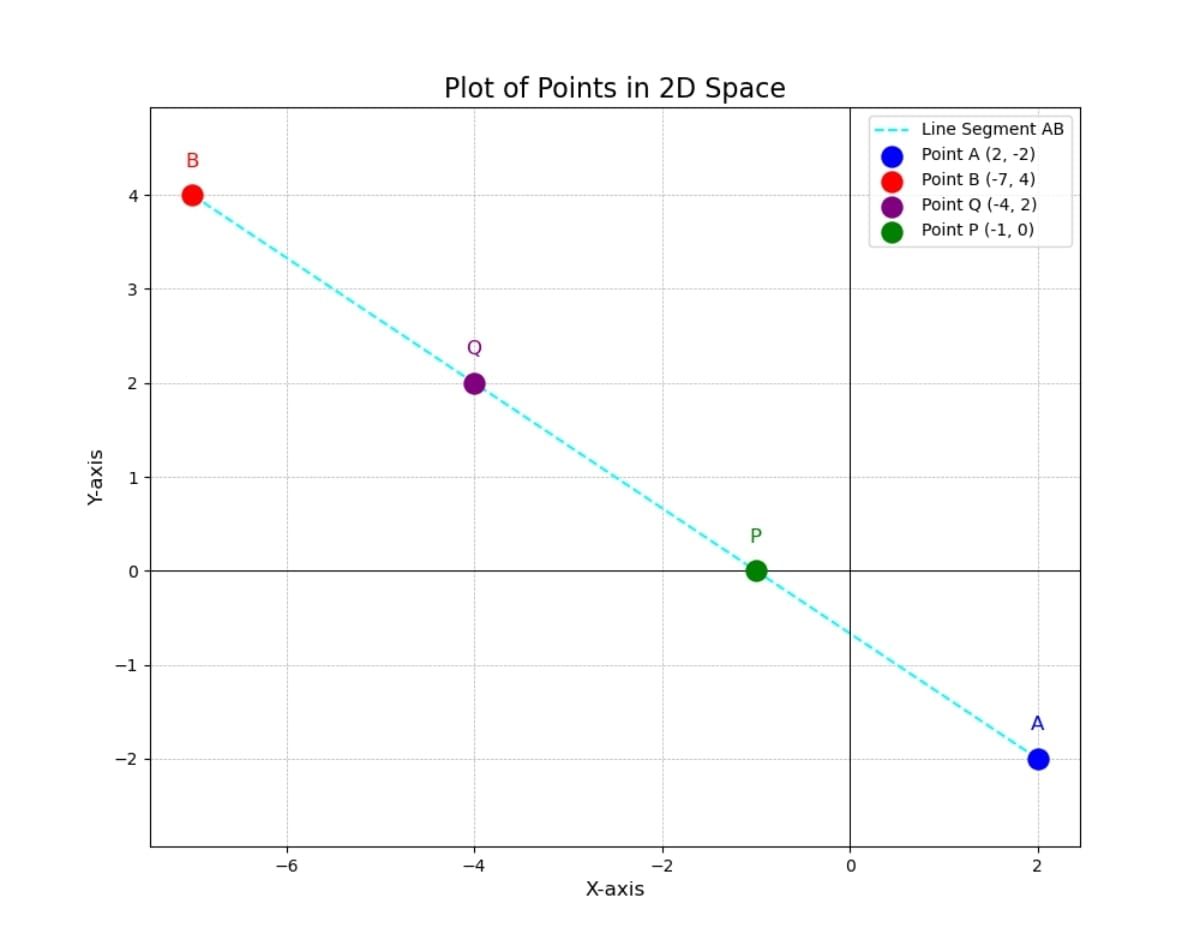
\includegraphics[width=1\columnwidth]{Figs/1.jpg}
    \caption{Figure for 1.5.26}
    \label{fig1}
\end{figure}


\end{document}






















